Secure remote computation (Figure~\ref{fig:remote_computation}) is the problem
of executing software on a remote computer \textbf{owned and maintained by an
untrusted party}, with some integrity and confidentiality guarantees. In the
general setting, secure remote computation is an unsolved problem. Fully
Homomorphic Encryption~\cite{gentry2009fhe} solves the problem for a limited
family of computations, but has an impractical performance overhead
\cite{naehrig2011can}.

\begin{figure}[hbt]
  \centering
  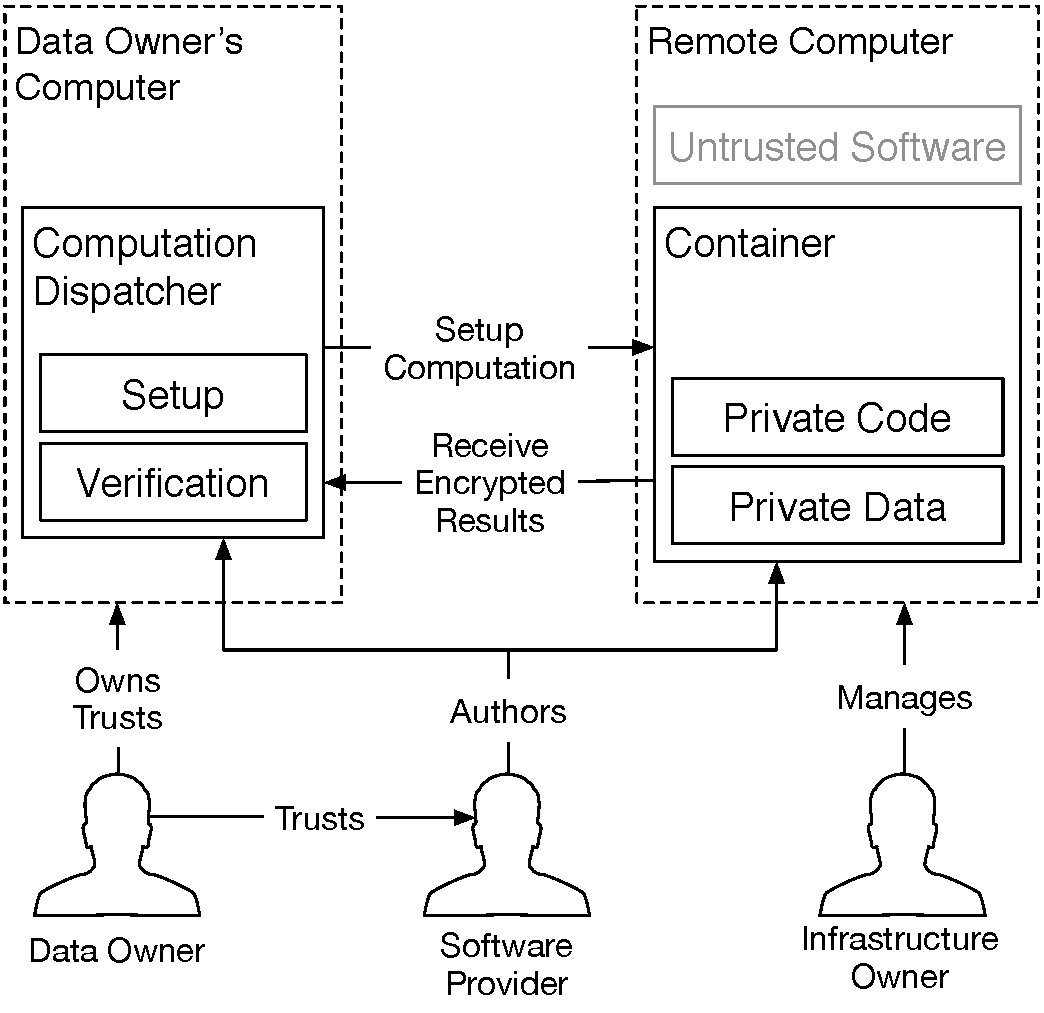
\includegraphics[width=75mm]{figures/remote_computation.pdf}
  \caption{
    Secure remote computation. A user relies on a remote computer, owned by an
    untrusted party, to perform some computation on her data. The user has some
    assurance of the computation's integrity and confidentiality.
  }
  \label{fig:remote_computation}
\end{figure}
